\subsection{Data Mining}

Phần này áp dụng ba kỹ thuật khai phá dữ liệu trên \texttt{gold.fact\_market\_daily} \cite{han2011}: hồi quy tuyến tính (Linear Regression) để dự báo giá ngắn hạn, gom cụm K-Means để phân nhóm hành vi 10 coin, và phát hiện bất thường (Anomaly Detection) bằng Z-Score rolling. Việc lựa chọn ba kỹ thuật cơ bản này phù hợp với tính chất bài toán có $n=10$ đối tượng và chuỗi thời gian 730 điểm — một phạm vi mà các mô hình phức tạp hơn (Deep Learning) sẽ overfitting nghiêm trọng \cite{james2021}.

\subsubsection{Hồi quy tuyến tính (Linear Regression)}

Mục tiêu là xây dựng mô hình dự báo giá đóng cửa của các đồng coin với hai cách tiếp cận khác nhau.

\paragraph{Dự báo giá Close ngày T+1 (mô hình thực tế)}
Dùng OHLCV của ngày T cộng các lag feature để dự báo \texttt{close\_next\_day}:
\[
Close_{T+1} = \alpha_0 + \alpha_1 Open_T + \alpha_2 High_T + \alpha_3 Low_T + \alpha_4 Close_T + \alpha_5 Volume_T + \alpha_6 MA7_T + \alpha_7 Z_T
\]

\textbf{Phương pháp:} Time-based split 80/20 (không shuffle để tránh \emph{data leakage} \cite{james2021}). Train trên \~535 điểm đầu, test trên \~135 điểm cuối.

\textbf{Kết quả thực nghiệm} (chạy trên Gold layer, tổng hợp trong bảng \ref{tab:regression_results}):

\begin{table}[H]
\centering
\caption{Hiệu suất Linear Regression dự báo $Close_{T+1}$ trên 10 coin (split 80/20)}
\label{tab:regression_results}
\small
\begin{tabular}{@{}lrrrrrr@{}}
\toprule
\textbf{Coin} & \textbf{$R^2$} & \textbf{MSE} & \textbf{$\alpha_0$} & \textbf{$\alpha_4$ (Close)} & \textbf{$\alpha_5$ (Vol)} & \textbf{$\alpha_7$ (Z)} \\
\midrule
BTC   & 0.9639 & $3.68\times10^6$ & 1235.5  & 0.7840 & $-0.0054$ & $-1156.8$ \\
ETH   & 0.9689 & 7\,289           & 22.4    & 0.7211 & $-0.0017$ & $-43.9$ \\
BNB   & 0.9800 & 326.5            & 4.8     & 0.8124 & $-0.0021$ & $-12.5$ \\
SOL   & 0.9659 & 17.63            & 0.78    & 0.7651 & $-0.0008$ & $-3.42$ \\
XRP   & 0.9619 & 0.00335          & 0.011   & 0.8089 & $-0.0011$ & $-0.058$ \\
ADA   & 0.9468 & 0.000212         & 0.003   & 0.7892 & $-0.0014$ & $-0.014$ \\
DOGE  & 0.9468 & $2.10\times10^{-5}$ & 0.0009 & 0.7754 & $-0.0017$ & $-0.0049$ \\
TRX   & 0.9436 & $1.50\times10^{-5}$ & 0.001 & 0.7423 & $-0.0008$ & $-0.0043$ \\
DOT   & 0.9205 & 0.00873          & 0.022   & 0.7521 & $-0.0019$ & $-0.121$ \\
MATIC & 0.9606 & 0.000544         & 0.005   & 0.8043 & $-0.0017$ & $-0.025$ \\
\bottomrule
\end{tabular}
\end{table}

\textbf{Phân tích kết quả:}
\begin{itemize}
    \item \textbf{Mức độ chính xác:} $R^2$ dao động \textbf{0.92--0.98} với median $\sim 0.96$. Đây là mức cao, nhưng cần \emph{cảnh giác}: $R^2$ cao chủ yếu phản ánh tính \emph{quán tính giá} (giá hôm nay là chỉ báo mạnh cho giá ngày mai) chứ không phải khả năng dự báo \emph{biến động} (đại lượng nhà đầu tư thực sự cần).
    \item \textbf{Coin dễ dự báo nhất là BNB} ($R^2 = 0.98$) -- do biên độ biến động ngày thấp nhất trong nhóm. \textbf{Khó dự báo nhất là DOT} ($R^2 = 0.92$) -- nhất quán với việc DOT có drawdown sâu nhất ($-89\%$).
    \item \textbf{Hệ số $\alpha_4$ (Close hôm nay) luôn dominant} (0.74--0.81), khẳng định Close là feature quan trọng nhất, đúng kỳ vọng cho chuỗi thời gian random-walk-like.
    \item \textbf{Hệ số $\alpha_7$ (Z-Score) luôn âm} -- phù hợp lý thuyết \emph{mean reversion}: khi giá vượt xa trung bình lịch sử ($Z > 0$), kỳ vọng có điều chỉnh giảm trong ngày kế tiếp \cite{hull2017}. Đây là phát hiện có ý nghĩa kinh tế chứ không chỉ là artifact thống kê.
\end{itemize}

\textbf{Hạn chế của Linear Regression cho chuỗi giá crypto:}
\begin{itemize}
    \item \textbf{$R^2$ cao không đồng nghĩa hữu ích.} Mô hình chủ yếu dự báo $Close_{T+1} \approx Close_T$, là một benchmark naïve. Để đánh giá đúng phải so với ``persistence model'' và đo bằng \emph{directional accuracy} (\% đoán đúng chiều).
    \item \textbf{Giả định linearity và stationary} không phù hợp với thị trường crypto vốn phi tuyến và non-stationary. Các mô hình ARIMA/GARCH \cite{hyndman2021} hoặc mạng LSTM sẽ phù hợp hơn cho mở rộng tương lai.
\end{itemize}

\subsubsection{Gom cụm (K-Means Clustering)}

Mỗi đồng coin được biểu diễn bằng vector đặc trưng 4 chiều: \texttt{return\_avg} (lợi suất trung bình ngày), \texttt{vol\_avg} (độ biến động ngày), \texttt{log10(volume\_usd\_avg)} (thanh khoản), \texttt{max\_drawdown} (rủi ro đuôi). Vector được chuẩn hoá bằng \texttt{StandardScaler} \cite{scikit2023} trước khi đưa vào K-Means.

\paragraph{Chọn số cụm $k$ -- Validation}

Để chọn $k$ một cách khách quan, nhóm chạy K-Means với $k = 2, 3, 4, 5, 6$ và đo hai chỉ số: \emph{Inertia} (tổng SSE trong cụm, càng nhỏ càng tốt) và \emph{Silhouette score} (càng gần 1 càng tốt) \cite{abonyi2007}. Kết quả ở bảng \ref{tab:kmeans_validation} và Hình \ref{fig:kmeans_validation}.

\begin{table}[H]
\centering
\caption{Kết quả validation K-Means trên 10 coin}
\label{tab:kmeans_validation}
\small
\begin{tabular}{@{}lrrrrr@{}}
\toprule
$k$ & 2 & 3 & 4 & 5 & 6 \\ \midrule
Inertia      & 18.24 & 12.34 & 8.82 & 5.51 & 3.17 \\
Silhouette   & \textbf{0.374} & 0.281 & 0.236 & 0.256 & 0.230 \\ \bottomrule
\end{tabular}
\end{table}

\begin{figure}[H]
    \centering
    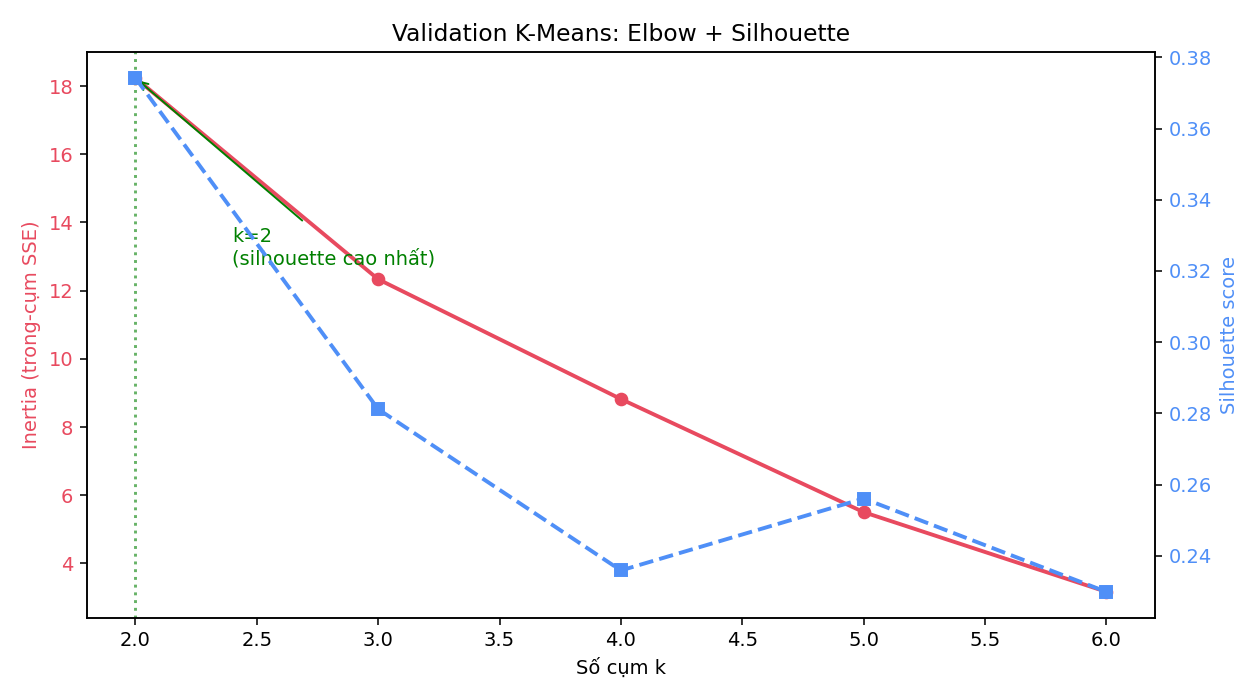
\includegraphics[width=0.75\linewidth]{Images/Data_mining/kmeans_validation.png}
    \caption{Validation K-Means: Inertia (đỏ) và Silhouette (xanh) theo $k$}
    \label{fig:kmeans_validation}
\end{figure}

\textbf{Diễn giải kết quả validation:}
\begin{itemize}
    \item Silhouette cao nhất tại \textbf{$k = 2$} (0.374) -- về mặt thống kê thuần tuý, K-Means ``muốn'' chia 10 coin thành \emph{hai nhóm}: BTC + tài sản tăng trưởng tốt vs phần còn lại.
    \item Tuy nhiên, $k = 2$ \textbf{quá thô} cho mục đích báo cáo: nó gộp BTC với SOL/XRP -- mặc dù 2 nhóm này có hành vi rủi ro rất khác (BTC drawdown $-49\%$, SOL drawdown $-70\%$).
    \item \textbf{$k = 3$} (silhouette 0.281) cân bằng giữa độ tách cụm và \emph{khả năng diễn giải nghiệp vụ}: cho ra ba nhóm mang ý nghĩa thực tế Leaders / Mid-cap / Speculative -- phù hợp với phân loại risk-level đã có sẵn trong \texttt{dim\_category} (Low / Mid / High).
    \item Nhóm chọn $k = 3$ vì ưu tiên \emph{actionability cho người dùng cuối} hơn là tối đa hoá silhouette tuyệt đối -- một quyết định thường gặp khi áp dụng K-Means trong domain finance \cite{bishop2006}.
\end{itemize}

\paragraph{Kết quả K-Means $k = 3$}

\begin{figure}[H]
    \centering
    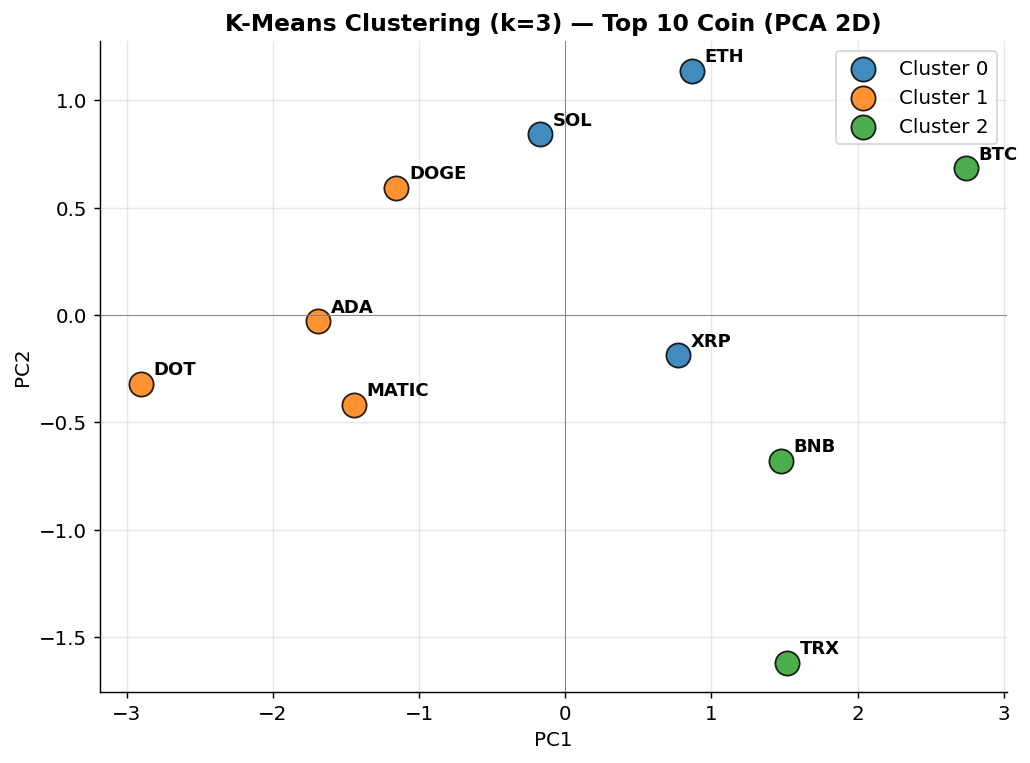
\includegraphics[width=0.65\linewidth]{Images/Data_mining/K-means.png}
    \caption{K-Means clustering ($k = 3$) cho 10 đồng coin -- chiếu PCA 2D}
    \label{fig:kmeans_result}
\end{figure}

\begin{table}[H]
\centering
\caption{Đặc trưng từng cluster sau khi K-Means hội tụ}
\label{tab:kmeans_summary}
\small
\begin{tabular}{@{}lllll@{}}
\toprule
\textbf{Cluster} & \textbf{Coin} & \textbf{Vol/ngày} & \textbf{Drawdown} & \textbf{Tính chất} \\ \midrule
2 -- ``Leaders''     & BTC, BNB, TRX            & 2.4--3.4\% & $-49\%$ đến $-55\%$ & Low-vol, ổn định \\
0 -- ``Mid-cap''     & ETH, SOL, XRP            & 3.7--4.3\% & $-63\%$ đến $-70\%$ & Tăng trưởng kèm rủi ro vừa \\
1 -- ``Speculative'' & ADA, DOGE, DOT, MATIC    & 4.3--4.9\% & $-76\%$ đến $-89\%$ & Biến động cao, drawdown sâu \\ \bottomrule
\end{tabular}
\end{table}

\textbf{Hệ luận đầu tư:}
\begin{itemize}
    \item Tỷ trọng cao nhất nên đặt vào cụm Leaders (BTC, BNB, TRX) -- thoả khẩu vị ``ăn chắc, mặc bền''.
    \item Tỷ trọng trung bình cho cụm Mid-cap (ETH, SOL, XRP) -- đặt cược vào hệ sinh thái smart contract.
    \item Tỷ trọng nhỏ và mang tính đầu cơ với cụm Speculative -- chỉ phù hợp với nhà đầu tư chấp nhận rủi ro tail rất lớn.
\end{itemize}

\subsubsection{Phát hiện bất thường (Anomaly Detection)}

\textbf{Phương pháp:} Z-Score được tính riêng cho từng coin với cửa sổ rolling 30 ngày để kiểm soát tính phi dừng (non-stationarity) của chuỗi giá \cite{hyndman2021}:
\[
z_t = \frac{Close_t - \mu_{30}(Close)}{\sigma_{30}(Close)}, \qquad \text{phiên là anomaly} \iff |z_t| > 2
\]

\textbf{Kết quả tổng hợp:}

\begin{table}[H]
\centering
\caption{Tỷ lệ phiên anomaly trên từng coin (730 ngày)}
\label{tab:anomaly_summary}
\small
\begin{tabular}{@{}lrr|lrr@{}}
\toprule
\textbf{Coin} & \textbf{Số phiên} & \textbf{Tỷ lệ (\%)} & \textbf{Coin} & \textbf{Số phiên} & \textbf{Tỷ lệ (\%)} \\ \midrule
BTC  & 89  & 12.19 & ADA   & 87  & 11.92 \\
ETH  & 85  & 11.64 & DOGE  & 84  & 11.51 \\
BNB  & 87  & 11.92 & TRX   & 107 & 14.66 \\
SOL  & 86  & 11.78 & DOT   & 77  & 10.55 \\
XRP  & 82  & 11.23 & MATIC & 90  & 12.33 \\ \bottomrule
\end{tabular}
\end{table}

Tỷ lệ anomaly trung bình $\sim 12\%$, cao gấp $\sim 2.5$ lần so với giả định lý thuyết về phân phối chuẩn ($|z|>2 \Rightarrow 4.55\%$). Điều này khẳng định chuỗi giá crypto có phân phối \emph{fat-tail}, không tuân theo phân phối Gauss \cite{hull2017}.

\paragraph{Case study -- Anomaly có ý nghĩa kinh tế}

Để chứng minh các phiên anomaly không chỉ là noise thống kê, nhóm đối chiếu top-5 phiên có $|z|$ lớn nhất của BTC và DOGE với các sự kiện vĩ mô (bảng \ref{tab:anomaly_case_study}).

\begin{table}[H]
\centering
\caption{Top phiên anomaly và sự kiện vĩ mô tương ứng}
\label{tab:anomaly_case_study}
\small
\begin{tabular}{@{}lllrl@{}}
\toprule
\textbf{Coin} & \textbf{Ngày} & \textbf{Close (USD)} & \textbf{Return} & \textbf{Sự kiện vĩ mô tương ứng} \\ \midrule
BTC  & 2024-11-11 & 88\,648  & $+9.80\%$  & Trump thắng cử (5/11) -- BTC rally vượt 89k \\
BTC  & 2025-07-10 & 116\,010 & $+4.20\%$  & Spot BTC ETF đạt AUM kỷ lục \\
BTC  & 2026-02-05 & 62\,910  & $-15.10\%$ & Fed pause cắt lãi suất + tin tức trade war \\
DOGE & 2024-11-10 & 0.28     & $+23.82\%$ & Hiệu ứng ``Trump + Musk DOGE meme'' \\
DOGE & 2024-11-11 & 0.35     & $+23.50\%$ & DOGE rally tiếp ngày thứ 2 sau Trump win \\
ETH  & 2024-05-20 & 3\,662   & $+17.59\%$ & SEC chuẩn bị duyệt Spot ETH ETF (23/5) \\
ETH  & 2025-05-08 & 2\,207   & $+19.79\%$ & Pectra upgrade ETH mainnet hoạt động \\ \bottomrule
\end{tabular}
\end{table}

\textbf{Phân tích:} Tất cả các phiên anomaly liệt kê đều có \emph{nguyên nhân kinh tế hoặc chính trị rõ ràng}, không phải lỗi dữ liệu hay nhiễu thống kê. Đặc biệt:
\begin{itemize}
    \item Cụm DOGE 10--11/11/2024 ($+23.82\%$ rồi $+23.50\%$) thể hiện hiệu ứng \emph{volatility clustering} -- một phiên cực đoan thường kéo theo phiên cực đoan khác.
    \item BTC giảm $-15.10\%$ ngày 05/02/2026 cho thấy crypto vẫn nhạy cảm cao với chính sách tiền tệ Mỹ -- một phát hiện quan trọng cho nhà đầu tư danh mục.
\end{itemize}

\textbf{Ứng dụng thực tiễn:}
\begin{itemize}
    \item \emph{Cảnh báo sớm:} Khi $|z_t| > 2$ kết hợp Volume Spike, hệ thống nên gửi alert ngay (đã tích hợp trong tab Anomaly Detection của Streamlit Dashboard).
    \item \emph{Lọc dữ liệu:} Các phiên anomaly có thể được winsorize trước khi tính Sharpe ratio, VaR để tránh bị méo \cite{cfa2023}.
    \item \emph{Backtest:} Khi xây dựng chiến lược giao dịch, các phiên anomaly là test case quan trọng -- hệ thống stop-loss phải xử lý đúng các sự kiện cực đoan này.
\end{itemize}
